\section{Archive process implementation}
This section gives an overview for the architecture of the archive process that would be responsible
to move the project data to the Synology. 

\subsection{Components for the archive process}
An Archive in the MARS ecosystem is tedious due to its distributed architecture. The process requires communication between a many components for a 
successful run. Figure \ref{fig:archiveComponent} depicts the high level components and the interfaces that the archive requires. The Archive
component exposes an API (Section \ref{section:APIDesign}) via an external port to the client. 

The marking component includes interfaces to mark a project and unmark the project in case of failure. This component communicates with the marking service which
is responsible for marking all the resources. Also, the metadata, file, scenario, result configurations, sim plans and sim runs components get make a connection to 
their respective services get the corresponding data which would be stored in the Synology using the interface provided by the Synology component.

\subsubsection{Performance optimization for simulation results}
For better performance
the simulation results are archived  using a database dump provided by the interface that will be triggered using the archive simulation result component. 
Dumping the result data directly to the Synology increases the throughput of the Archive service by reducing the network calls and decreases the total data processing
time because it has to be processed only at one end i.e. Database utility service. For this purpose a dumping API endpoint will be implemented which would trigger the data dump process in the 
Synology. In addition, it can be argued why other external components (e.g. file service) do not have a direct dependency to the Synology as it would reduce more
processing times as well. One of the main goals of the Archive service is also to act as an abstraction layer for the archives and in case of future changes the
connection interface must only be changed in inside the Archive service instead of all the other services.

\begin{figure}[H]
    \centering 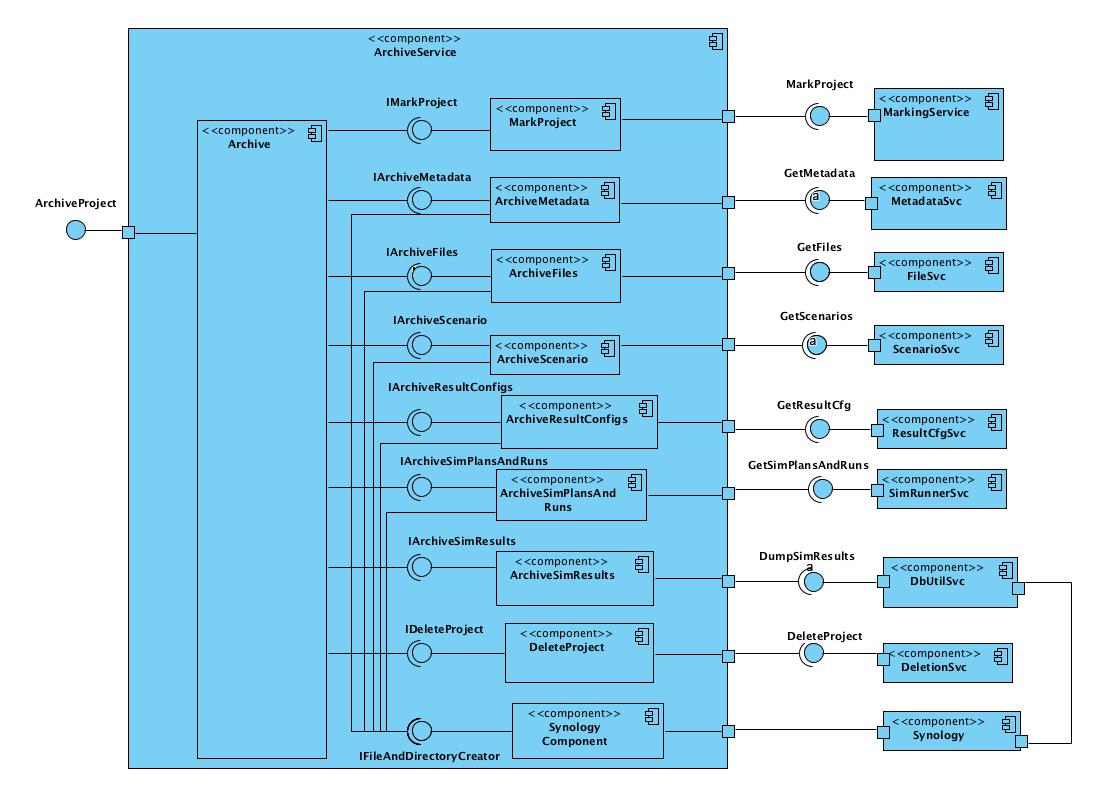
\includegraphics[scale=0.45]{grafiken/archiveComponent.png}
    \caption{Component Diagram for the Archive process}
    \label{fig:archiveComponent}
\end{figure}



\begin{figure}[H]
    \centering 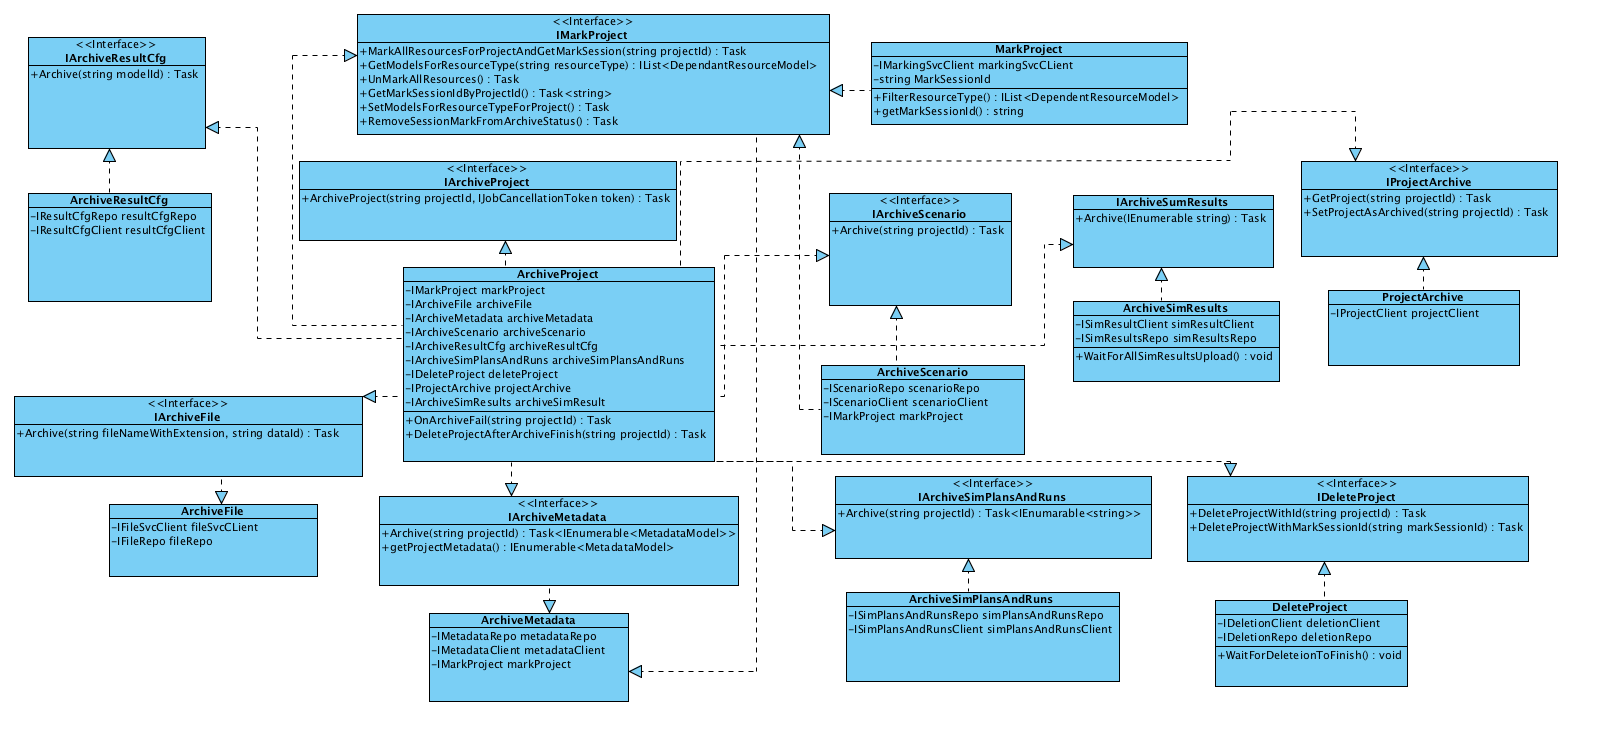
\includegraphics[height=6.5cm, angle=90, origin=c, width=11cm]{grafiken/archiveClassDiagram.png}
    \caption{Class Diagram for the Archive process (Component level)}
    \label{fig:archiveClassDiagram}
\end{figure}

Figure \ref{fig:archiveClassDiagram} illustrates the class diagram for the archive process. This diagram attempts to depict only the top level components
which perform a certain action (e.g. archiving files, archiving simulation result). The archive process is is a complex 
task, thus involves a lot of operations and communications. The operations include HTTP Get request to an external service, a repository storing the received
data in to the Synology and forwarding the received data to the next component which requires it. This involves more sub classes which cannot be illustrated in a single diagram. 

\subsubsection{Repository Pattern implementation}
It is seen that many components require access to the Synology storage to archive their respective data, presenting the problem of having data duplication
persistence logic in many components. To solve this the repository pattern will be implemented where there would be a abstraction layer i.e. repository which
provides the query interface to the component (See Appendix). This abstraction layer would be injected to the required components and they can just call the 
method to carry out persistence actions. In addition, this also decouples the component from the type of storage being used i.e. Synology, so it would not
matter for the component if the type of storage is changed from Synology to something else since it just needs the interface for persistence. Figure 
\ref{fig:repositoryPattern} illustrates how the repository acts as an abstraction layer for the client aiding the system to be more cohesive.
 
\begin{figure}[H]
    \centering 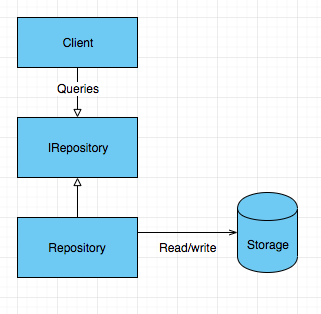
\includegraphics[scale=0.7]{grafiken/repositoryPattern.png}
    \caption{Repository Pattern overview}
    \label{fig:repositoryPattern}
\end{figure}


\newpage
\begin{figure}[H]
    \centering 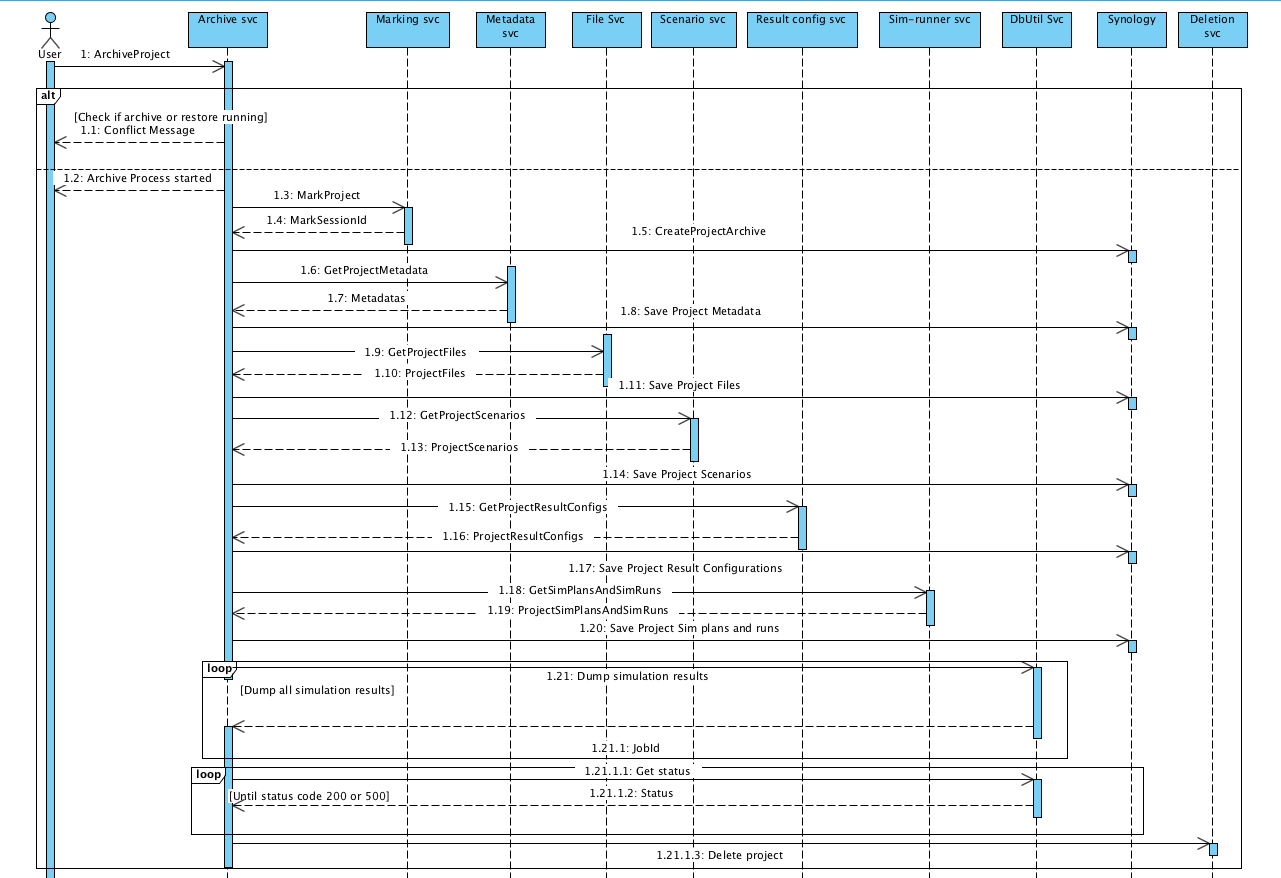
\includegraphics[scale=0.5, angle=90, origin=c]{grafiken/sequenceArchive.png}
    \caption{Sequence Diagram for the Archive process}
    \label{fig:sequenceArchive}
\end{figure}

Figure \ref{fig:sequenceArchive} illustrates the Sequence diagram for an complete archive process. The first step after an archive request would be to check
whether an archive or retrieve process for the current project is under progress. In case the process is in progress the archive request would be denied to the
user with an conflict message. If no processes are running then an archive job (a separate thread) would be created and a message to the client with start of archive process would be
sent. Following the job creation the project will be marked so that during archive no changes to the project resources could be made. If this step fails the archive 
process would stop logging the error. After marking step completes the archive process receives a mark session id and the dependent resources which would allow the process to make
changes to the resources. Using the dependent resources the process retrieves metadata, files, scenarios, result configurations, simulation plans, simulation runs 
respectively and persists them in synology. Lastly, the simulation result dump action will be requested which will archive the result data. The process waits until
all the result data is archived successfully. After a successful archive a request to delete the project data would be made so that the system memory can be freed.

\subsubsection{Future possibility of failure recovery with snapshot}
It can be noticed from the sequence diagram that the resources are being persisted right after they are successfully retrieved rather than a bulk operation
(e.g. sequence number 1.8 in Figure \ref{fig:sequenceArchive}). This
is implemented considering a possibility that in the near future the archive service would archive the project as a snapshot. In case of archive failure the process
could be resumed from the snapshot in contrast to the current atomic implementation of the process.

